\documentclass{article}


% if you need to pass options to natbib, use, e.g.:
%     \PassOptionsToPackage{numbers, compress}{natbib}
% before loading neurips_2023


% ready for submission
\usepackage[preprint]{neurips_2023}


% to compile a preprint version, e.g., for submission to arXiv, add add the
% [preprint] option:
%     \usepackage[preprint]{neurips_2023}


% to compile a camera-ready version, add the [final] option, e.g.:
%     \usepackage[final]{neurips_2023}


% to avoid loading the natbib package, add option nonatbib:
%    \usepackage[nonatbib]{neurips_2023}


\usepackage[utf8]{inputenc} % allow utf-8 input
\usepackage[T1]{fontenc}    % use 8-bit T1 fonts
\usepackage{hyperref}       % hyperlinks
\usepackage{url}            % simple URL typesetting
\usepackage{booktabs}       % professional-quality tables
\usepackage{amsfonts}       % blackboard math symbols
\usepackage{nicefrac}       % compact symbols for 1/2, etc.
\usepackage{microtype}      % microtypography
\usepackage{xcolor}         % colors
\usepackage{graphicx}
\usepackage{subcaption}
\usepackage{algpseudocode}
\usepackage{algorithm}

\title{Theory and Methods for the Ferromagnetic Ising Model}


% The \author macro works with any number of authors. There are two commands
% used to separate the names and addresses of multiple authors: \And and \AND.
%
% Using \And between authors leaves it to LaTeX to determine where to break the
% lines. Using \AND forces a line break at that point. So, if LaTeX puts 3 of 4
% authors names on the first line, and the last on the second line, try using
% \AND instead of \And before the third author name.


\author{
    Jay Shen \\
    Department of Physics \\
    University of Chicago\\
    Chicago, IL 60637 \\
    \texttt{jshe@uchicago.edu} \\
    \And
    Mark Lee \\
    Department of Statistics \\
    University of Chicago\\
    Chicago, IL 60637 \\
    \texttt{markyl@uchicago.edu} \\
}


\begin{document}

\graphicspath{ {../graphics} }

\maketitle

\begin{abstract}

The Ising model is a historically important problem in statistical mechanics 
\cite{lenz1920}. 
Although it was originally proposed as a crude approximation of magnetic 
phenomena, it furnished statistical mechanics, and later probabilistic science 
as whole, with a new paradigm of graph-based modeling that would prove 
influential.
Especially in the distilled, theoretical study of probabilistic graphical 
models (PGMs), which today is its own field, many methods developed for Ising 
models and spin-glasses—as well as the rich physical vocabulary of energies, 
entropy, and partition functions—have been repurposed and reinterpreted for 
application towards diverse problems \cite{koller}. 

In this paper, we pay homage to the Ising model by applying modern computational 
solutions to the original problem of magnetism. 
We discuss the theory of the Ising model from a physical perspective, and 
examine its correspondence with PGMs theory. 
We then evaluate two approaches to inference—Markov Chain Monte Carlo and
belief propagation—and discuss their strengths and weaknesses when appplied to 
predict physical phenomena. 
%
%
%
%
%
\end{abstract}
%
%
%
%
%
\section{Theory of the Ising Model}

The prevailing physical theory explains magnetism as a consequence of the 
intrinsic spin all particles possess \cite{griffiths}. 
This spin produces a magnetic dipole moment $\vec{\mu}$ proportional to the 
spin $\sigma$:
\[\vec{\mu} = \mu \sigma\]
If an external magnetic field $\vec{B}$ is present, the potential energy is 
given by the classical formula:
\[U_B = - \vec{\mu} \cdot \vec{B}\]
Handily, this also absorbs the splitting of atomic energy levels at the quantum 
mechanical level. 

There also exist pairwise exchange interactions between particles due to the 
mutual effects of their magnetic moments.
These exchange effects have strengths defined by constants $J_{ij}$. 
The potential energy contained by these pairwise interactions is:
\[U_{ij} = - J_{ij} \vec{\mu_i} \cdot \vec{\mu_j}\]
We will ignore quantum mechanical spin-spin coupling and exclusion energies. 

Note that both potential energies are minimized when the moments align with 
$\vec{B}$ and with each other. 
This corresponds to the theory of ferromagnetism as a systematic alignment of 
spins. 

Now, consider a collection of particles $\vec{\mu_i}$ in the prescence of an 
external magnetic field $\vec{B}$. 
The Hamiltonian, which specifies the total energy of the system, is defined by 
the sum of all pairwise and unary energies:
\begin{equation}\label{eq:exactE}
    E(\vec{\mu}) = -\frac{1}{2}\sum_i \sum_j J_{ij} \vec{\mu_i} \cdot \vec{\mu_j} - \sum_i \vec{\mu_i} \cdot \vec{B}
\end{equation}
In most cases, working with this Hamiltonian is intractable. 
Luckily, we can simplify it by making several strategic assumptions. 

First, in the context of an atomic lattice, all relevant particles are fermionic 
and have spin-$\frac{1}{2}$ up or down. 
We assume that all particles within an atom have identical spin, so the spin of 
each atom as a whole is fermionic. 
Then the magnetic moments simplify to $\vec{\mu_i} = \mu \sigma_i$, where 
$\sigma_i \in \{-1, 1\}$ is the atomic spin. 

Second, we make a mean-field nearest-neighbor approximation. 
That is, we assume strength of pairwise interactions is negligible for 
non-adjacent pairs. 
We also assume the non-negligible $J_{ij}$'s are equal to some $J$, that is, 
that the material is organized in some regular lattice. 

Coalescing constants, the Hamiltonian reduces nicely to:
\begin{equation}\label{eq:isingE}
    E(\vec{\sigma}) = -J\sum_i \sum_{j \in adj(i)} \sigma_i \sigma_j - \sum_i \sigma_i B_i
\end{equation}
Given this energy expression, we can use the Boltzmann distribution to compute a 
probability of some microstate $\vec{\sigma}$ at inverse temperature $\beta$:
\begin{equation} \label{eq:boltzmann}
    P(\vec{\sigma}) = \frac{1}{Z}e^{-\beta E(\vec{\sigma})} 
\end{equation}
The physical theory of the Ising model has now been developed and we can turn to 
the purely abstract task of inference on a PGM. 
%
%
%
%
%
\section{Inference on Ising Models}
%
%
%
%
%
In many cases, the Ising model of ferromagnetism is used to produce physical 
measurables like energy and magnetization. 
For example, Ernst Ising's original inquiry asked if the Ising model was capable 
of demonstrating phase transitions in the magnetic state. 

Now, these measurables require marginal distributions in order to compute. 
For example, the quantities we are most interested in, the energy 
(\ref{eq:isingE}) and the magnetization ($\mathbb{E}[\sigma]$), both require 
explicit microstate spins. 
We will now examine two approaches to computing these marginals—Markov Chain 
Monte Carlo and belief propagation. 
%
%
%
%
%
\subsection{Markov Chain Monte Carlo}
%
%
%
%
%
Monte Carlo algorithms produce better and better estimates by repeated sampling 
from the true distribution. 
When the true distribution is not immediately available for sampling, employing 
Markov Chain Monte Carlo defines an approximate distribution that hopefully, 
during sampling, approaching the true one. 

In the context of the Ising model, the Markov states accessible from some 
microstate of spins $\vec{\sigma}$ are those created by flipping any spin 
$\sigma_i$ in $\vec{\sigma}$. 
We can sample from these adjacent microstates, then, by choosing a random 
$\sigma_i$ to flip. 
Since we want to move towards the true, equilibrium distribution, we only 
transition to the new sampled microstate $\vec{\sigma}'$ if 
$P(\vec{\sigma}') > P(\vec{\sigma})$. 
Using the formula for the Boltzmann distribution, this criterion is equivalent 
to $E(\vec{\sigma}') < E(\vec{\sigma})$. 

In practice, we will compute the change in energy 
$\Delta E = E(\vec{\sigma}') - E(\vec{\sigma})$, which has a nice form:
\[
    \Delta E = E(\vec{\sigma}') - E(\vec{\sigma}) = 2 \sigma_i (J \sum_{j \in adj(i)} \sigma_j + B_i)
\]
If $\Delta E < 0$, we transition states. 
If $\Delta E \geq 0$, we will transition microstates with probability defined by 
the Boltzmann factor:
\[
    \frac{P(\vec{\sigma}')}{P(\vec{\sigma})}
    = e^{-\beta \Delta E} 
\]
This nicely models the phenomena of spin flips caused by field fluctuations. 

We implemented this process in Python on square lattices of spins. 
For our sampling process, we iterated through all spins in random order, at each 
step evaluating the transition defined by flipping the present spin. 
We believe this best simulates the physical equilibration. 

\begin{figure}[h]
    \begin{subfigure}{\textwidth}
        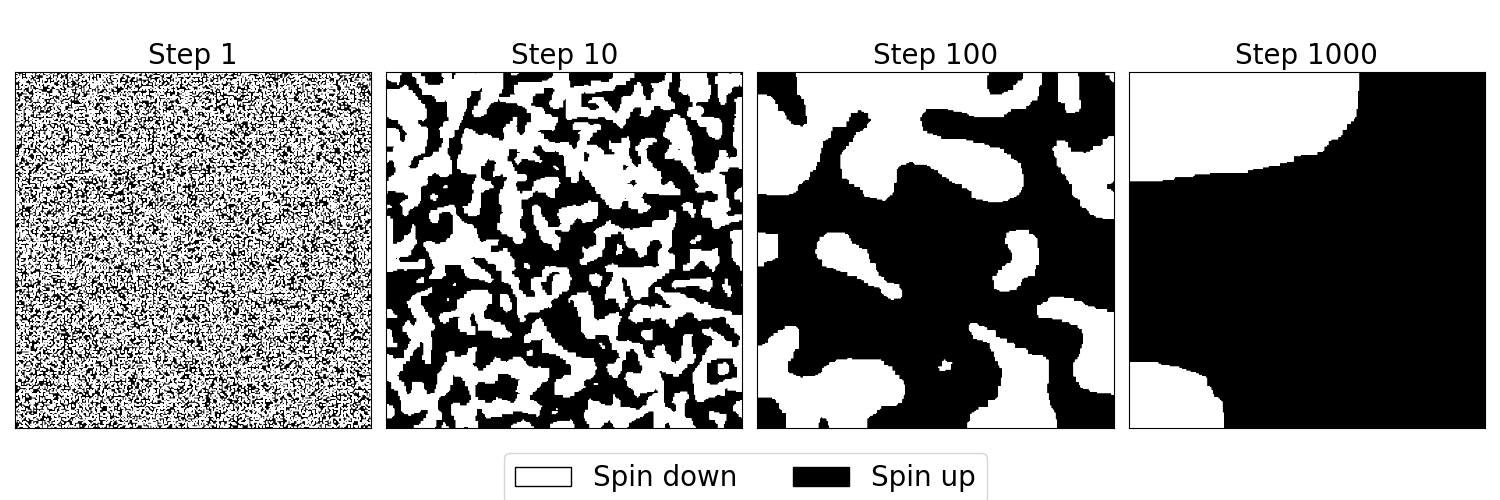
\includegraphics[width=\textwidth]{report_mcmc_gaussian}
        \centering
        \caption{\textit{
            Spin lattice sample microstates from various points in the sampling 
            process
        }}
        \label{fig:mcmc_gaussian_a}
    \end{subfigure}
    \begin{subfigure}{\textwidth}
        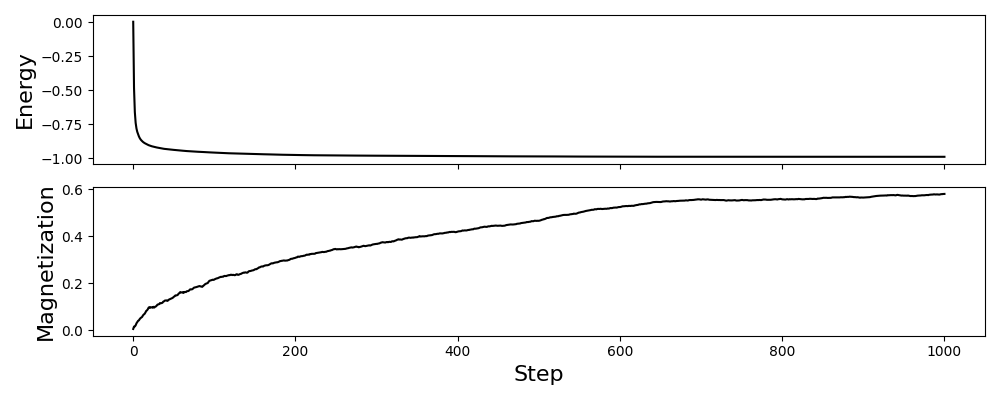
\includegraphics[width=\textwidth]{report_mcmc_gaussian_measurables}
        \centering
        \caption{\textit{Measurables of samples during the sampling process}}
        \label{fig:mcmc_gaussian_b}
    \end{subfigure}
    \centering
    \caption{\textit{
        MCMC quenching of an initial randomly generated $256 \times 256$ spin 
        lattice sample with $J = 0.5$, $\beta = 10$, and a centered Gaussian 
        magnetic field
        $B_{ij} = 0.01 \exp [-\frac{1}{1024}((i-128)^2 + (j-128)^2)]$. 
    }}
    \label{fig:mcmc_gaussian}
\end{figure}

In the MCMC quenching simulation conducted in \ref{fig:mcmc_gaussian}, we 
observe several expected phenomena. 
The pairwise interactions are exhibited by the clusters of aligned spins which 
form and coalesce as the number of steps grows. 
The prescence of the magnetic field also seems to magnetize the entire lattice, 
as indicated both by the convergence on full spin alignment in 
\ref{fig:mcmc_gaussian_a}, and the increasing magnetization measured in 
\ref{fig:mcmc_gaussian_b}. 

\begin{figure}
    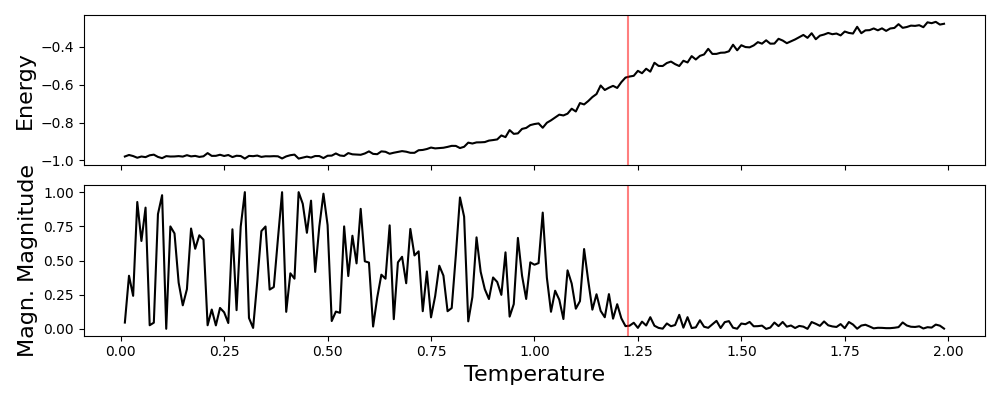
\includegraphics[width=\textwidth]{report_mcmc_phase}
    \caption{\textit{
        $100 \times 100$ spin lattice run with $J=0.5$, $\vec{B} = 0$ and 
        $T \in \{0.01, 0.02, \dots, 2\}$. 
        Note that $\beta = \frac{1}{T}$. 
        An hand-estimated Curie temperature is marked in red. 
    }}
    \label{fig:mcmc_phase}
\end{figure}

Using this MCMC inference scheme, we ran an experiment (Figure 
\ref{fig:mcmc_phase}) simulating the phase transitions expected of the 2D 
Ising model \cite{peirerls1936}. 

As seen, the energy and magnetization of the lattice both degenerate to zero 
as the temperature increases. 
The physical interpretation of this is that, at high temperatures, the field 
fluctuations which cause spin flips become more and more likely, and thus 
the alignment of spins is constantly being disrupted. 
It has been shown analytically that the Ising model in 2D exhibits this 
phenomenon of phase transitions. 
This simulation reinforces this claim. 
We can also identify what is called the Curie temperature, the point at which 
the phase transition occurs. 

%
%
%
%
%
\subsection{Belief Propagation}
%
%
%
%
%
Message-passing belief propagation algorithms are another way to estimate true 
marginals for general graphical models. 
They are derived from the theory of variable elimination, but are applicable to 
general graphs which may include cycles. 

Belief propagation is especially effective and simple to implement on Ising 
models. 
This follows from the Boltzmann distribution that defines the joint distribution 
of the Ising model:
\begin{equation}\label{isingJoint}
    \tilde{P}(\vec{\sigma}) = \exp \Bigr [\beta J\sum_i \sum_{j \in adj(i)} \sigma_i \sigma_j + \beta \sum_i \sigma_i B_i \Bigr ]
\end{equation}
It factorizes nicely over the graph representing the Ising lattice:
\begin{equation}\label{gibbsFactorization}
    \tilde{P}(\vec{\sigma}) = \prod_i \exp \Bigr [\beta \sigma_i B_i \Bigr ] \prod_{j \in adj(i)} \exp \Bigr [ \beta J \sigma_i \sigma_j \Bigr ]
\end{equation}
This defines a factor graph of node and edge potentials representing the unary 
and pairwise potentials, respectively:
\[
    \phi_i = \exp \Bigr [\beta \sigma_i B_i \Bigr ]
    \qquad \qquad
    \phi_{ij} = \exp \Bigr [ \beta J \sigma_i \sigma_j \Bigr ]
\]
We ran a belief propagation routine on the factor graph according to the update 
scheme in Algorithm \ref{alg:bp}. 

\begin{algorithm}
    \caption{Belief propagation calibration step on factor graph}
    \begin{algorithmic}[1]
        \Statex \underline{\textbf{Input}}
        \Statex \quad Factor graph: $G(V = \{v_i\}_i \cup \{v_{ij}\}_{i, j}, E)$
        \Statex \quad Unary Factors: $\{\phi_i(\sigma_i)\}_i$
        \Statex \quad Pairwise Factors: $\{\phi_{ij}(\sigma_i, \sigma_j)\}_{i, j}$

        \Statex \underline{\textbf{Output:}}
        \Statex \quad Unary beliefs: $\{\beta_i(\sigma_i)\}_i$
        \Statex \quad Pairwise beliefs: $\{\beta_{ij}(\sigma_i, \sigma_j)\}_{i, j}$
        
        \Statex // Pass messages from unary nodes
        \For{unary $v_i \in V$}
        \For{pairwise $v_{ij} \in Nb(v_i)$}
        \State $\delta[v_i \rightarrow v_{ij}] = \phi_i \prod_{k \neq j} \delta[v_{ik} \rightarrow v_i]$ \quad // Nothing to sum!
        \EndFor
        \EndFor

        \Statex // Pass messages from pairwise nodes
        \For{pairwise $v_{ij} \in V$}
        \For{$\{v_i, v_j\} = Nb(v_{ij})$}
        \State $\delta[v_{ij} \rightarrow v_i] = \sum_{v_j} \phi_{ij} \delta[v_j \rightarrow v_{ij}]$
        \State $\delta[v_{ij} \rightarrow v_j] = \sum_{v_i} \phi_{ij} \delta[v_i \rightarrow v_{ij}]$
        \EndFor
        \EndFor

        \Statex // Compute beliefs
        \For{unary $v_i \in V$}
        \State $\beta_i = \phi_i \prod_{j} \delta[v_{ij} \rightarrow v_i]$
        \EndFor
        \For{pairwise $v_{ij} \in V$}
        \State $\beta_{ij} = \phi_{ij} \delta[v_i \rightarrow v_{ij}] \delta[v_j \rightarrow v_{ij}]$
        \EndFor
        \State \textbf{return } $\{\beta_i\}_i, \{\beta_{ij}\}_{ij}$
    \end{algorithmic}
    \label{alg:bp}
\end{algorithm}

\begin{figure}
    \begin{subfigure}{\textwidth}
        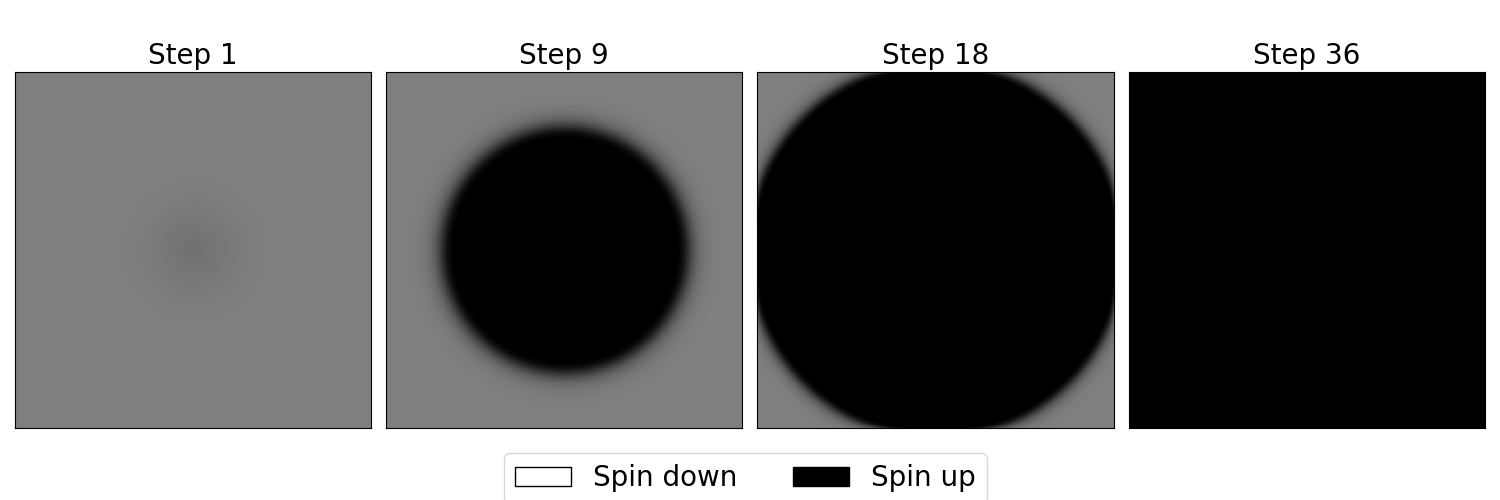
\includegraphics[width=\textwidth]{report_bp_gaussian}
        \centering
        \caption{\textit{
            Spin lattice marginal beliefs at various points in the calibration 
            process. 
        }}
        \label{fig:bp_gaussian_a}
    \end{subfigure}
    \begin{subfigure}{\textwidth}
        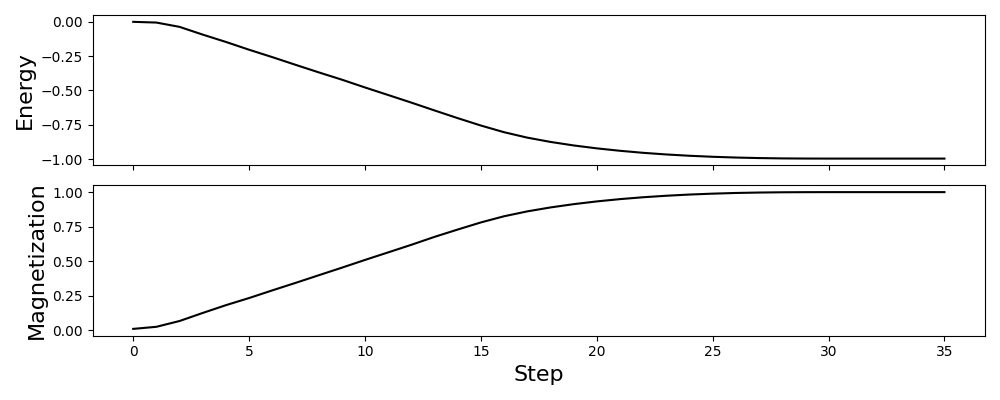
\includegraphics[width=\textwidth]{report_bp_gaussian_measurables}
        \centering
        \caption{\textit{Mean value of measurables taken from samples from marginals}}
        \label{fig:bp_gaussian_b}
    \end{subfigure}
    \centering
    \caption{\textit{
        Belief propagation to estimate marginal distributions of spin lattice 
        with $J = 0.5$, $\beta = 10$, and a centered Gaussian 
        magnetic field
        $B_{ij} = 0.01 \exp [-\frac{1}{1024}((i-128)^2 + (j-128)^2)]$. 
        We run belief propagation until the difference between messages falls 
        below $\epsilon = 0.001$. 
    }}
    \label{fig:bp_gaussian}
\end{figure}

We tested this on the same system from \ref{fig:mcmc_gaussian}. 
Algorithm \ref{alg:bp} is run repeatedly until the maximum change in the 
messages falls below some $\epsilon$. 
We also take measurements by taking samples from the marginal beliefs at 
each step and computing their mean energy and magnetization. 

After calibration, the approximate marginals visualized in Figure
\ref{fig:bp_gaussian_a} reflect what we would expect, full system spin alignment 
by the magnetic field. 
The trend in the magnetization is also observable in the plots of sample 
measurables, which reflect the appropriate minimization of energy. 

\subsection{Comparing MCMC and belief propagation}

When deciding which paradigm of inference to use for the Ising model, there are 
a number of considerations with respect to speed, output, interpretability, etc. 
Here, we will discuss these variables with respect to MCMC and belief 
propagation. 

MCMC is useful because it provides easy access to valid microstate samples 
throughout the estimation process. 
Importantly, this makes the computation of meaningful measurables easy and 
intuitive. 
This is a direct consequence of the simulatory nature of MCMC, which emulates, 
as closely as possible, the physical processes that underlie our desired 
statistics. 

Unfortunately, MCMC is slow, and very difficult to parallelize. 
This slowness is compounded by its tendency to follow unoptimal branches in the 
search tree and get stuck in local minima. 

Belief propagation, on the other hand, is useful because of the immediate access 
to highly-accurate marginal beliefs, upon calibration. 
Belief propagation is also fast. 
It is highly parallelizable, especially on factor graphs, and inherently 
bypasses many of the search tree inefficiencies that Monte Carlo methods 
struggle with. 

The downsides of belief propagation lie in the poor interpretability of 
intermediate steps. 
Since the marginal beliefs do not necessarily agree with each other until 
they are fully calibrated, they do not correspond to physically meaningful 
microstates when sampled. 
As a consequence, it is difficult to take measurements of the system without 
having to draw samples. 
Deriving macrostate properties from the partition function may be one solution, 
but we leave that problem to future studies. 

For most physical use cases, we conclude that MCMC is the better approach to 
inference. 
The interpretability and ease of measurements when dealing with explicit 
microstates is extremely valuable, especially in the context of magnetism. 
As we showed, simulating and analyzing physical phenomena such as phase 
transitions are straightforward and can be very precise. 
%
%
%
%
%
\section{Conclusions}
%
%
%
%
%
In this paper, we revisited the Ising model, an important probabilistic model of 
ferromagnetism, to pay homage and exercise our modern computational methods. 
We discussed the theory behind it, from a physics point of view, and linked it 
to the PGMs theory we use to perform inference on it. 
We evaluate two approaches, Markov Chain Monte Carlo and belief propagation, 
for marginal inference on the Ising model, and discussed their respective 
strengths and weaknesses. 

We concluded MCMC was the better approach in the context of the Ising model 
because of its strong interpretability and ease of measurement. 
These strengths enables us to demonstrate the phenomenon of magnetic phase 
transitions in a highly emulative way. 
However, for faster inference that is interested in the true equilibrium beliefs 
of the system, belief propagation may prove more effective. 

For the future, there is much to explore both with respect to the problem of 
magnetism as well as the Ising model. 
As an example, deriving beliefs about the values of macrostate measurables, 
which might involve the partition function, is an interesting and challenging 
task that might lessen our reliance on MCMC. 
We conclude by affirming the power and usefulness of the Ising model in the 
context of physical as well as abstract probabilistic modeling. 
Within its rich theory, we can intuit much about modern probabilistic 
reasoning and its connection with complex physical ensembles. 
And in its rich history, in the road from ferromagnetism to deep neural 
networks, we can find solace in the fact that our crude toy models might not be 
so childish after all. 
%
%
%
%
%
\bibliographystyle{unsrt}
\bibliography{references}

\end{document}